\documentclass[border=10pt]{standalone}
\usepackage{circuitikz}
\usepackage{tikz}
\usetikzlibrary{calc, positioning, arrows.meta}

\begin{document}
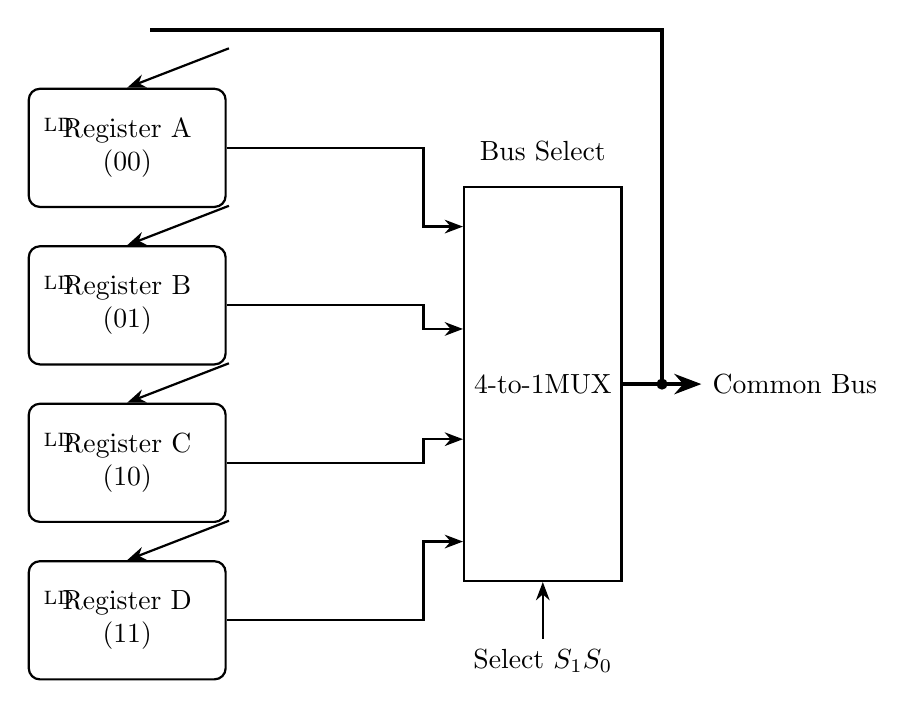
\begin{tikzpicture}[
    >=Stealth, 
    thick, 
    block/.style={draw, rectangle, minimum height=1.5cm, minimum width=2.5cm, fill=white, align=center, rounded corners},
    mux/.style={draw, trapezium, trapezium angle=75, minimum height=3cm, shape border rotate=270, fill=white, align=center},
    label_font/.style={font=\small}
]

    % Registers A, B, C, D
    \node[block] (regA) at (0, 6) {Register A\\(00)};
    \node[block] (regB) at (0, 4) {Register B\\(01)};
    \node[block] (regC) at (0, 2) {Register C\\(10)};
    \node[block] (regD) at (0, 0) {Register D\\(11)};

    % MUX (Abstracted as a single 4x1 MUX block for the "System")
    % In reality it's 4 MUXes for 4 bits, but for system view we show one block handling the data bus.
    \node[draw, fill=white, minimum width=2cm, minimum height=5cm, right=3cm of regB, yshift=-1cm] (mux) {4-to-1\\MUX};

    % MUX Inputs
    \draw[->] (regA.east) -| ($(mux.west) + (-0.5, 2.0)$) -- ($(mux.west) + (0, 2.0)$);
    \draw[->] (regB.east) -| ($(mux.west) + (-0.5, 0.7)$) -- ($(mux.west) + (0, 0.7)$);
    \draw[->] (regC.east) -| ($(mux.west) + (-0.5, -0.7)$) -- ($(mux.west) + (0, -0.7)$);
    \draw[->] (regD.east) -| ($(mux.west) + (-0.5, -2.0)$) -- ($(mux.west) + (0, -2.0)$);

    % Select Lines
    \node (sel) at ($(mux.south) + (0, -1)$) {Select $S_1 S_0$};
    \draw[->] (sel) -- (mux.south);

    % Bus Output
    \draw[->, line width=1.5pt] (mux.east) -- ++(1, 0) node[right] {Common Bus};

    % Logic Flow (Abstract)
    % Showing that Bus connects back to inputs of registers.
    \coordinate (bus_tap) at ($(mux.east) + (0.5, 0)$);
    \node[circ] at (bus_tap) {};
    
    % Draw feedback path to top
    \draw[line width=1.5pt] (bus_tap) -- ++(0, 4.5) -- ++(-6.5, 0) coordinate (top_left);
    
    % Drop downs to registers inputs (Load)
    \foreach \reg in {regA, regB, regC, regD} {
        \draw[->] (top_left |- \reg.north) ++(1.0, 0.5) -- (\reg.north);
        \node[above right=0.1cm of \reg.west, font=\scriptsize] {LD};
    }
    
    % Annotations
    \node[above=0.2cm of mux] {Bus Select};

\end{tikzpicture}
\end{document}
